\documentclass[11pt]{article}
\usepackage[utf8]{inputenc}
\usepackage[english]{babel}
\usepackage{graphicx}
\usepackage[numbers]{natbib}

\graphicspath{{pics/}}

\DeclareUnicodeCharacter{00A0}{ }


\title{KRKPA7 problem in various data mining tools \\ 4IZ451 - Knowledge discovery in databases}
\author{Tomáš Maršálek}
\date{\today}

\begin{document}
\maketitle
\thispagestyle{empty}
\clearpage

\section{Introduction}
The purpose of this work is to analyze database of KRKPA7 problem using four different data mining tools. Some of the chosen data mining programs are freely available (Weka) or freely available for non-commercial use (RapidMiner) or proprietary licensed (Enterprise Modeler, IBM PASW). %% TODO je to tak do řitě?
The nature of problem for this assignment is suitable for classification and association modeling, but not for clustering.

\section{KRKPA7 problem}
KRKPA7 is a shorthand for King Rook versus King Pawn on A7, which is a chess endgame. The black player has a king and a pawn left, where the pawn is on A7, which is one turn away from turning him into a queen. The white player has a turn in this situation and has a king and a rook to play with.

\begin{figure}[!ht]
	\centering
	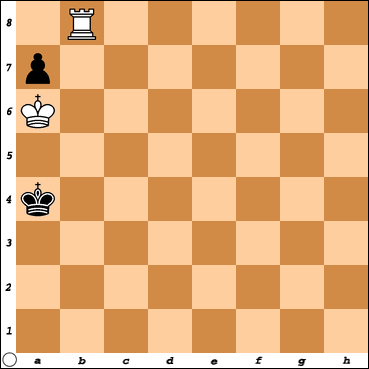
\includegraphics[width=.7\textwidth]{example}
	\caption{Example board setup}
\end{figure}

\clearpage

\subsection{Data set}
Data set contains 3196 setups of chess board, each one with different positions
of both kings and the rook, the pawn is fixed on A7. The 37th column is a class
column denoting {\bf win} or {\bf nowin} of white player. For our purposes we
don't need to perform any preprocessing. The set is not as large for the
algorithms to be unable to create desired models.

Each board setup is described by 36 attributes described in table \ref{tab:attributes}.
\begin{table}[h]
\makebox[\textwidth][c]{
\begin{tabular}{|l|l|l|}
\hline
{\bf Position} & {\bf Abbreviation} & {\bf description} \\
\hline
1	&bkblk	&the BK is not in the way \\
2	&bknwy	&the BK is not in the BR's way \\
3	&bkon8	&the BK is on rank 8 in a position to aid the BR \\
4	&bkona	&the BK is on file A in a position to aid the BR \\
5	&bkspr	&the BK can support the BR \\
6	&bkxbq	&the BK is not attacked in some way by the pro- moted WP \\
7	&bkxcr	&the BK can attack the critical square (b7) \\
8	&bkxwp	&the BK can attack the WP \\
9	&blxwp	&B attacks the WP (BR in direction x = -1 only) \\
10	&bxqsq	&one or more Black pieces control the queening square \\
11	&cntxt	&the WK is on an edge and not on a8 \\
12	&dsopp	&the kings are in normal opposition \\
13	&dwipd	&the WK distance to intersect point is too great \\
14	&hdchk	&there is a good delay because there is a hidden check \\
15	&katri	&the BK controls the intersect point \\
16	&mulch	&B can renew the check to good advantage \\
17	&qxmsq	&the mating square is attacked in some way by the promoted WP \\
18	&r2ar8	&the BR does not have safe access to file A or rank 8 \\
19	&reskd	&the WK can be reskewered via a delayed skewer \\
20	&reskr	&the BR alone can renew the skewer threat \\
21	&rimmx	&the BR can be captured safely \\
22	&rkxwp	&the BR bears on the WP (direction x = -1 only) \\
23	&rxmsq	&the BR attacks a mating square safely \\
24	&simpl	&a very simple pattern applies \\
25	&skach	&the WK can be skewered after one or more checks \\
26	&skewr	&there is a potential skewer as opposed to fork \\
27	&skrxp	&the BR can achieve a skewer or the BK attacks the WP \\
28	&spcop	&there is a special opposition pattern present \\
29	&stlmt	&the WK is in stalemate \\
30	&thrsk	&there is a skewer threat lurking \\
31	&wkcti	&the WK cannot control the intersect point \\
32	&wkna8	&the WK is on square a8 \\
33	&wknck	&the WK is in check \\
34	&wkovl	&the WK is overloaded \\
35	&wkpos	&the WK is in a potential skewer position \\
36	&wtoeg	&the WK is one away from the relevant edge \\
\hline
\end{tabular}
}
\caption{Board positions attributes~\citep{Michie1995-MICCAA-2}}
\label{tab:attributes}
\end{table}

\clearpage

\section{WEKA}
WEKA (Waikato Environment for Knowledge Analysis) is an open source data mining software from University od Waikato, New Zealand. 

\subsection{Classification}
In order to predict whether the white player wins or loses from board setup, we
tested several classification algorithms implemented in WEKA. Classifiers were trained using k-fold cross-validation with $k = 10$.

\paragraph{ZeroR} is a simple classifier which ignores every attribute and
simply assigns dominating class to each sample.  Uneffective in this case
because the distribution of win and nowin class is roughly equal (52.2215\% win
and 47.7785\% nowin).
\paragraph{OneR} is a classifier which selects attribute with smallest
classification error and uses that attribute as its classification rule.
\paragraph{NaiveBayes} is a classifier constructed from naive Bayes probability model.
\paragraph{Decision tree algorithms} construct a decision tree from the attributes of training set.

\mbox{}\\
\begin{table}[h]
\makebox[\textwidth][c]{
\begin{tabular}{|l|r|}
\hline
{\bf Algorithm} & {\bf Success rate} \\
\hline
ZeroR & 52.2215\% \\
OneR &  66.4581\% \\
NaiveBayes &  87.8911\% \\
J48 (decision tree) & 99.4368\% \\
SimpleCart (decision tree) & 99.3742\% \\
RandomForest (decision tree) & 98.7797\% \\
\hline
\end{tabular}
}
\caption{WEKA Classifiers}
\label{tab:attributes}
\end{table}

\subsection{Association}
To find association rules in KRKPA7 data set we used {\bf Apriori} algorithm.
Best rules found:

\begin{enumerate}
\item thrsk=f 3060 $\rightarrow$ spcop=f 3060
\item skach=f thrsk=f 3049 $\rightarrow$ spcop=f 3049
\item hdchk=f thrsk=f 3045 $\rightarrow$ spcop=f 3045
\item reskd=f thrsk=f 3045 $\rightarrow$ spcop=f 3045
\item skach=f 3185 $\rightarrow$ spcop=f 3184
\item hdchk=f 3181 $\rightarrow$ spcop=f 3180
\item reskd=f 3170 $\rightarrow$ spcop=f 3169
\item hdchk=f skach=f 3170 $\rightarrow$ spcop=f 3169
\item reskd=f skach=f 3159 $\rightarrow$ spcop=f 3158
\item hdchk=f reskd=f 3155 $\rightarrow$ spcop=f 3154
\end{enumerate}


\clearpage
\section{Rapid Miner}
RapidMiner is a software by company RapidMiner for commercial use of machine learning, data and text mining and predictive and business analytics.

\subsection{Classification}
Preprocessing steps for krkpa7 data set in RapidMiner require to only specify
target column.  To create a classifier in RapidMiner, we layout several
components together starting from data input, then going through validation
step, which makes all the partitioning, classification and model performance
evaluation, and finishing in the output of the pipeline.

\begin{figure}[!ht]
	\centering
    \makebox[\textwidth][c]{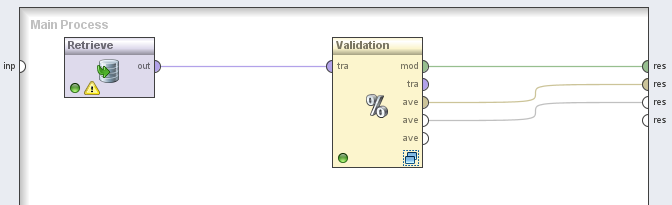
\includegraphics[width=1.2\textwidth]{rapid_main}}
    \caption{Pipeline setup}
\end{figure}

\begin{figure}[!ht]
	\centering
    \makebox[\textwidth][c]{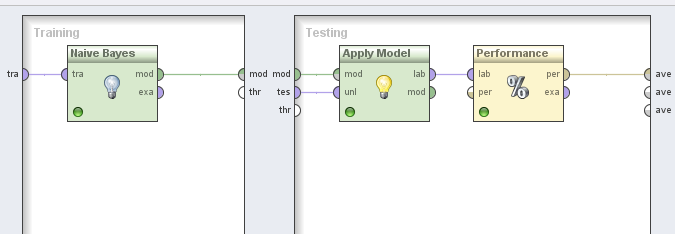
\includegraphics[width=1.2\textwidth]{rapid_naivebayes}}
    \caption{Naive bayes classifier component}
\end{figure}

If we use desicion tree classifier, we can get either graphical or textual
representation of the resulting classifier. We only include text formatted tree
below, because graphical representation was simply too wide to fit the page.


\mbox{} \\[1cm]
\small\begin{verbatim}
Tree
rimmx = f
|   bxqsq = f
|   |   wknck = f
|   |   |   wkna8 = f
|   |   |   |   bkxbq = f
|   |   |   |   |   wkpos = f
|   |   |   |   |   |   katri = b
|   |   |   |   |   |   |   bkblk = f: nowin {won=0, nowin=15}
|   |   |   |   |   |   |   bkblk = t
|   |   |   |   |   |   |   |   hdchk = f: won {won=21, nowin=1}
|   |   |   |   |   |   |   |   hdchk = t: nowin {won=0, nowin=4}
|   |   |   |   |   |   katri = n
|   |   |   |   |   |   |   bkblk = f
|   |   |   |   |   |   |   |   wkcti = f: nowin {won=0, nowin=55}
|   |   |   |   |   |   |   |   wkcti = t
|   |   |   |   |   |   |   |   |   r2ar8 = f
|   |   |   |   |   |   |   |   |   |   reskr = f
|   |   |   |   |   |   |   |   |   |   |   dsopp = f: nowin {won=2, nowin=3}
|   |   |   |   |   |   |   |   |   |   |   dsopp = t: won {won=2, nowin=0}
|   |   |   |   |   |   |   |   |   |   reskr = t: nowin {won=0, nowin=6}
|   |   |   |   |   |   |   |   |   r2ar8 = t: nowin {won=0, nowin=14}
|   |   |   |   |   |   |   bkblk = t
|   |   |   |   |   |   |   |   hdchk = f: won {won=22, nowin=0}
|   |   |   |   |   |   |   |   hdchk = t: nowin {won=0, nowin=4}
|   |   |   |   |   |   katri = w: won {won=50, nowin=0}
|   |   |   |   |   wkpos = t
|   |   |   |   |   |   katri = b
|   |   |   |   |   |   |   bkblk = f: nowin {won=0, nowin=20}
|   |   |   |   |   |   |   bkblk = t
|   |   |   |   |   |   |   |   rxmsq = f: won {won=8, nowin=0}
|   |   |   |   |   |   |   |   rxmsq = t: nowin {won=1, nowin=1}
|   |   |   |   |   |   katri = n
|   |   |   |   |   |   |   rxmsq = f
|   |   |   |   |   |   |   |   dsopp = f: won {won=221, nowin=0}
|   |   |   |   |   |   |   |   dsopp = t
|   |   |   |   |   |   |   |   |   dwipd = g
|   |   |   |   |   |   |   |   |   |   skewr = f: won {won=8, nowin=0}
|   |   |   |   |   |   |   |   |   |   skewr = t
|   |   |   |   |   |   |   |   |   |   |   wtoeg = n: won {won=3, nowin=0}
|   |   |   |   |   |   |   |   |   |   |   wtoeg = t: nowin {won=0, nowin=2}
|   |   |   |   |   |   |   |   |   dwipd = l: won {won=23, nowin=0}
|   |   |   |   |   |   |   rxmsq = t
|   |   |   |   |   |   |   |   qxmsq = f: nowin {won=0, nowin=15}
|   |   |   |   |   |   |   |   qxmsq = t: won {won=27, nowin=0}
|   |   |   |   |   |   katri = w: won {won=49, nowin=0}
|   |   |   |   bkxbq = t: won {won=599, nowin=0}
|   |   |   wkna8 = t
|   |   |   |   bknwy = f: nowin {won=0, nowin=106}
|   |   |   |   bknwy = t
|   |   |   |   |   r2ar8 = f
|   |   |   |   |   |   simpl = f: won {won=3, nowin=0}
|   |   |   |   |   |   simpl = t: nowin {won=0, nowin=5}
|   |   |   |   |   r2ar8 = t: nowin {won=0, nowin=9}
|   |   wknck = t
|   |   |   r2ar8 = f
|   |   |   |   bkxcr = f
|   |   |   |   |   skrxp = f
|   |   |   |   |   |   mulch = f
|   |   |   |   |   |   |   thrsk = f
|   |   |   |   |   |   |   |   bkona = f
|   |   |   |   |   |   |   |   |   reskr = f
|   |   |   |   |   |   |   |   |   |   blxwp = f
|   |   |   |   |   |   |   |   |   |   |   bkon8 = f
|   |   |   |   |   |   |   |   |   |   |   |   skach = f: won {won=38, nowin=0}
|   |   |   |   |   |   |   |   |   |   |   |   skach = t: nowin {won=0, nowin=2}
|   |   |   |   |   |   |   |   |   |   |   bkon8 = t: nowin {won=0, nowin=2}
|   |   |   |   |   |   |   |   |   |   blxwp = t: nowin {won=0, nowin=3}
|   |   |   |   |   |   |   |   |   reskr = t: nowin {won=0, nowin=6}
|   |   |   |   |   |   |   |   bkona = t: nowin {won=0, nowin=6}
|   |   |   |   |   |   |   thrsk = t: nowin {won=0, nowin=7}
|   |   |   |   |   |   mulch = t: nowin {won=0, nowin=18}
|   |   |   |   |   skrxp = t: nowin {won=0, nowin=34}
|   |   |   |   bkxcr = t: nowin {won=0, nowin=77}
|   |   |   r2ar8 = t
|   |   |   |   wkovl = f
|   |   |   |   |   bkxcr = f
|   |   |   |   |   |   bkona = f
|   |   |   |   |   |   |   mulch = f
|   |   |   |   |   |   |   |   bkon8 = f: won {won=8, nowin=0}
|   |   |   |   |   |   |   |   bkon8 = t: nowin {won=0, nowin=3}
|   |   |   |   |   |   |   mulch = t: nowin {won=0, nowin=11}
|   |   |   |   |   |   bkona = t: nowin {won=0, nowin=19}
|   |   |   |   |   bkxcr = t: nowin {won=0, nowin=41}
|   |   |   |   wkovl = t: nowin {won=0, nowin=295}
|   bxqsq = t: nowin {won=0, nowin=743}
rimmx = t: won {won=584, nowin=0}
\end{verbatim}


\clearpage


\section{IBM SPSS Modeler}
Originally named Clementine, also known as SPSS Clementine, PASW Modeler is a
data mining and text analytics software by IBM.

\subsection{Classification}
In the pipeline schema we first retrieve data from a file. Unlike in WEKA and
RapidMiner, we need to provide a csv file instead of more suitable arff file,
which contains more detailed definitions of data types. We run the data through
auto data preparation step and feed the result to feature selector. After the
selector is trained in the first run of the pipeline, we use the resulting
component in the next step of pipeline and feed the refined data to a partition
step so that we get two sets used for training and testing of the upcoming
models. In this case we used c5 decision tree and neural network classifiers.
Same as in the feature selector component, we need first to build the models
and use the newly created components down in the pipeline. To evaluate results
(c5 decision tree in table \ref{tab:c5_pasw} and neural net in table
\ref{tab:neural_pasw}) we feed the outputs from the classifiers to error
matrices for each of the models.


\begin{figure}[!ht]
	\centering
    \makebox[\textwidth][c]{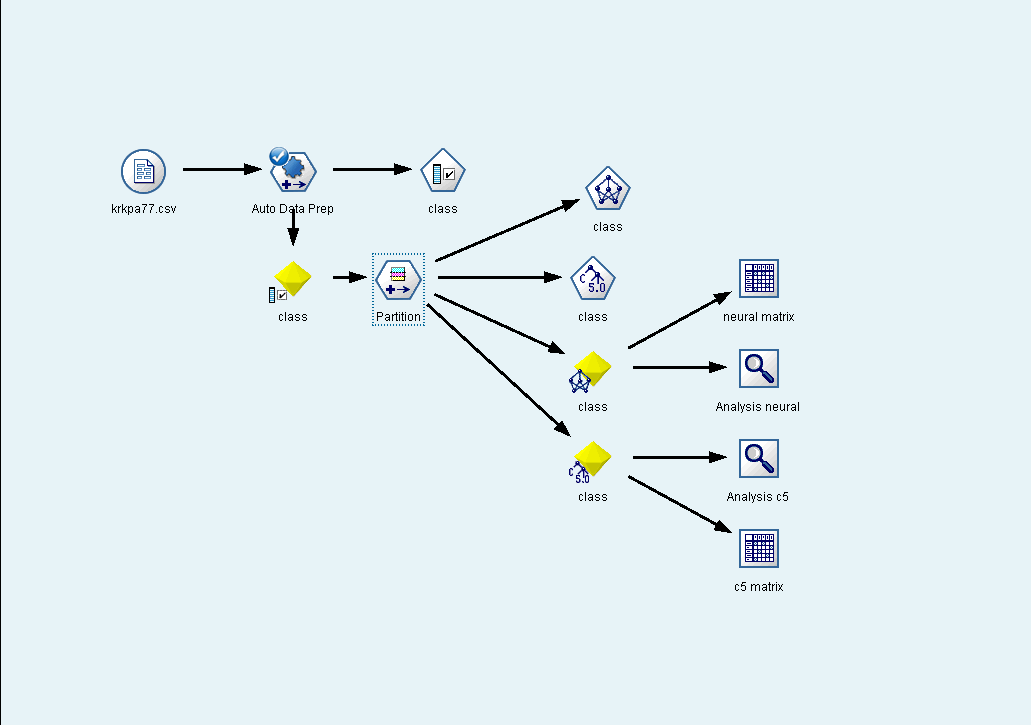
\includegraphics[width=1.2\textwidth]{pasw}}
    \caption{Pipeline setup of classifiers in PASW}

\end{figure}

\begin{figure}[!ht]
	\centering
    \makebox[\textwidth][c]{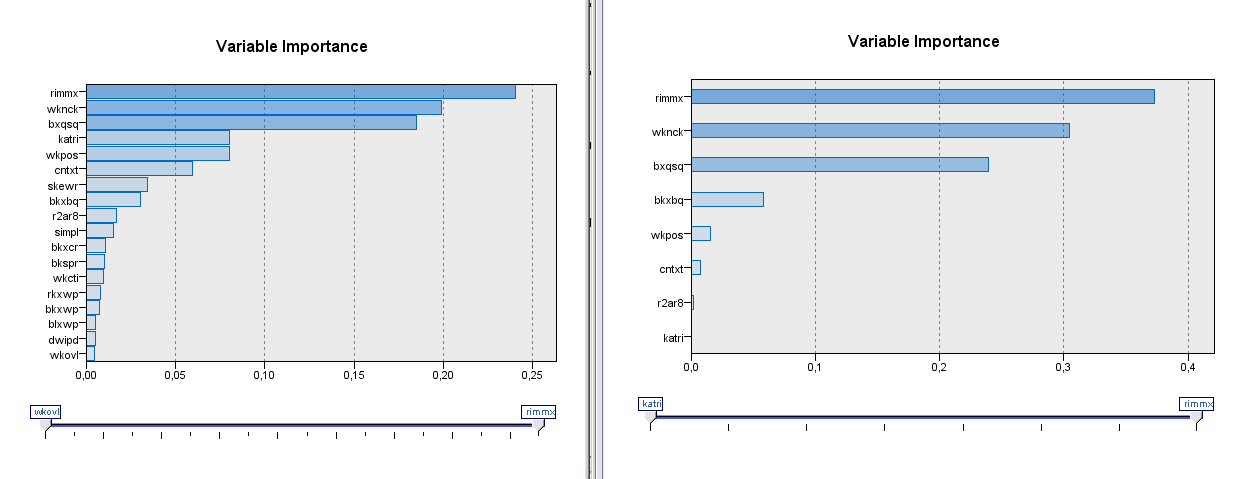
\includegraphics[width=1.3\textwidth]{pasw_models}}
    \caption{Result of PASW Models}
\end{figure}

\mbox{}\\
\begin{table}[h]
\makebox[\textwidth][c]{
\begin{tabular}{|c|l|r|}
\hline
{\bf class} & {\bf nowin} & {\bf win} \\
\hline
nowin & 1510 & 17 \\
won & 95 & 1574 \\
\hline
\end{tabular}
}
\caption{Error matrix for c5 decision tree in PASW}
\label{tab:c5_pasw}
\end{table}


\mbox{}\\
\begin{table}[h]
\makebox[\textwidth][c]{
\begin{tabular}{|c|l|r|}
\hline
{\bf class} & {\bf nowin} & {\bf win} \\
\hline
nowin & 1495 & 32 \\
won & 83 & 1586 \\
\hline
\end{tabular}
}
\caption{Error matrix for neural network in PASW}
\label{tab:neural_pasw}
\end{table}


\begin{figure}[!ht]
	\centering
\begin{verbatim}
Results for output field  class 
	Comparing $C- class  with  class 
		'Partition'            1_Training            2_Testing         
		Correct                     1 450   96,09%       1 634   96,86%
		Wrong                          59    3,91%          53    3,14%
		Total                       1 509                1 687
\end{verbatim}
\caption{Analysis of c5 decision tree in PASW}
\end{figure}


\begin{figure}[!ht]
	\centering
\begin{verbatim}
Results for output field  class 
	Comparing $N- class  with  class 
		'Partition'            1_Training            2_Testing         
		Correct                     1 457   96,55%       1 624   96,27%
		Wrong                          52    3,45%          63    3,73%
		Total                       1 509                1 687         
\end{verbatim}
\caption{Analysis of neural network in PASW}
\end{figure}


\clearpage


\section{SAS Enterprise Miner}
SAS (Statistical Analysis System) is a software suite by SAS Institute, which
offers both programming language capabilities through SAS programming language
and point-and-click interface for non-programmers.

For purposes of this project the point-and-click interface was used resulting
in diagram depicted in picture~\ref{pic:sas_diagram}.

\begin{figure}[!ht]
	\centering
    \makebox[\textwidth][c]{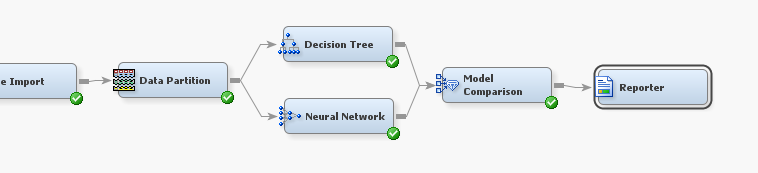
\includegraphics[width=1.2\textwidth]{sas_diagram}}
    \caption{SAS pipeline setup}
    \label{pic:sas_diagram}
\end{figure}

Same as in the previous pipeline-designer tools, we first create file importer
and load it with krkpag csv input file. The class column is marked as target
and the rest is kept as an input (picture~\ref{pic:sas_settarget}).

\begin{figure}[!ht]
	\centering
    \makebox[\textwidth][c]{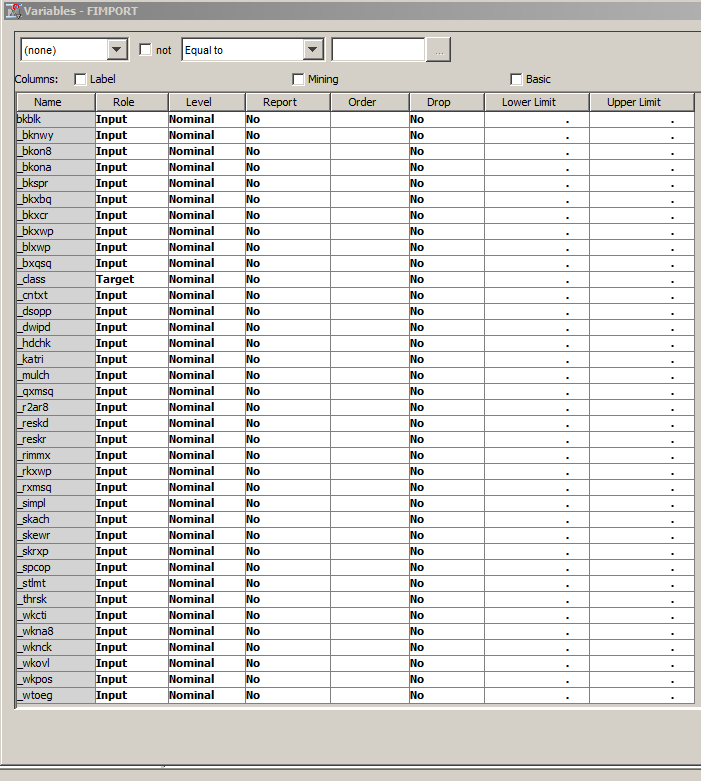
\includegraphics[width=1.0\textwidth]{sas_settarget}}
    \caption{SAS set target attribute}
    \label{pic:sas_settarget}
\end{figure}

\clearpage

We run the data through data partitioner in default ratio 40:30:30
(Training:Validation:Test) to two models - neural network and decision tree
with all the settings kept at defaults. The final stage of the pipeline before
reporting results is a model comparison box, which allows us to compare
generated models. We push output of this comparison to reporting output which
generates a nice pdf file with various data from which we are now only
interested in the error matrix for both classifiers and overall performance of
the models.

\begin{table}[h]
\makebox[\textwidth][c]{
\begin{tabular}{|l|l|l|l|l|l|}
\hline
{\bf Model} & {\bf Data Role} & {\bf False Negative} & {\bf True Negative} & {\bf False Positive} & {\bf True Positive} \\
\hline
Neural Network & TRAIN    &    8     &    603    &     8    &     659 \\
Neural Network & VALIDATE &   13     &    448    &    10    &     488 \\
Decision Tree  & TRAIN    &   13     &    556    &    55    &     654 \\
Decision Tree  & VALIDATE &   16     &    415    &    43    &     485 \\
\hline
\end{tabular}
}
\caption{SAS error matrices}
\label{tab:sas_error}
\end{table}


\begin{table}[h]
\makebox[\textwidth][c]{
\begin{tabular}{|l|l|l|}
\hline
{\bf Model} & {\bf Missclassification rate (valid)} & {\bf Average squared Error (valid) } \\
\hline
Neural Network & 0.023983 & 0.021215 \\
Decision Tree  & 0.061522 & 0.055342 \\
\hline
\end{tabular}
}
\caption{SAS model performance}
\label{tab:sas_performance_valid}
\end{table}

\begin{table}[h]
\makebox[\textwidth][c]{
\begin{tabular}{|l|l|l|}
\hline
{\bf Model} & {\bf Average squared error (train)} & {\bf Missclassification rate (train)} \\
\hline
Neural Network & 0.010720 & 0.012520 \\
Decision Tree  & 0.047754 & 0.053208 \\
\hline
\end{tabular}
}
\caption{SAS model performance}
\label{tab:sas_performance_train}
\end{table}

\clearpage


\section{Conclusion}
We used four data mining tools to show how to perform simple data
classification from KRKPA7 data set. We also used WEKA to further analyse the
data resulting in a set of association rules among attributes of the data set.
The purpose of this project was rather educational to make students familiar
with data mining tools both freely available and commercial.

Personally I found all of the tools intuitive to some degree because solving
the same problem in one tool makes you understand what to look for in the next
tool from the four. 

SAS left an impression on me. It is de facto industry standard even though
nowadays we have tools like R or numerical Python which are way less heavy on
licensing costs, but still not fully adopted by businesses in advanced data
analysis compared to SAS.

If I were to choose a data mining tool for my personal purposes I would choose
WEKA for the simple reason that it complies with ideas of open software which
according to me governs the way of evolution of software these days. It is
worth mentioning that it can be used as a library rather than rigidly using it
as a heavyweight GUI all-in-one tool that badly integrates with custom
software.

\subsection{Results}
Principles of used algorithms are basically equal in each of the used data
mining tools, therefore the accuracy of same algorithm models across different
tools is unsurprisingly very similar.

\bibliographystyle{csplainnat}
\bibliography{ref}

\end{document}
